\documentclass[12pt]{report}
\usepackage[utf8]{inputenc}
\usepackage[russian]{babel}
%\usepackage[14pt]{extsizes}
\usepackage{listings}
\usepackage{graphicx}
\usepackage{amsmath,amsfonts,amssymb,amsthm,mathtools} 

% Для листинга кода:
\lstset{ %
language=python,                 % выбор языка для подсветки (здесь это С)
basicstyle=\small\sffamily, % размер и начертание шрифта для подсветки кода
numbers=left,               % где поставить нумерацию строк (слева\справа)
numberstyle=\tiny,           % размер шрифта для номеров строк
stepnumber=1,                   % размер шага между двумя номерами строк
numbersep=5pt,                % как далеко отстоят номера строк от подсвечиваемого кода
showspaces=false,            % показывать или нет пробелы специальными отступами
showstringspaces=false,      % показывать или нет пробелы в строках
showtabs=false,             % показывать или нет табуляцию в строках
frame=single,              % рисовать рамку вокруг кода
tabsize=2,                 % размер табуляции по умолчанию равен 2 пробелам
captionpos=t,              % позиция заголовка вверху [t] или внизу [b] 
breaklines=true,           % автоматически переносить строки (да\нет)
breakatwhitespace=false, % переносить строки только если есть пробел
escapeinside={\#*}{*)}   % если нужно добавить комментарии в коде
}

% Для измененных титулов глав:
\usepackage{titlesec, blindtext, color} % подключаем нужные пакеты
\definecolor{gray75}{gray}{0.75} % определяем цвет
\newcommand{\hsp}{\hspace{20pt}} % длина линии в 20pt
% titleformat определяет стиль
\titleformat{\chapter}[hang]{\Huge\bfseries}{\thechapter\hsp\textcolor{gray75}{|}\hsp}{0pt}{\Huge\bfseries}


% plot
\usepackage{pgfplots}
\usepackage{filecontents}
\usetikzlibrary{datavisualization}
\usetikzlibrary{datavisualization.formats.functions}
\begin{filecontents}{LevM.dat}
3 2
4 3
5 3
6 5
7 6
\end{filecontents}

\begin{filecontents}{DamLevM.dat}
3 4
4 5
5 3
6 5
7 6
\end{filecontents}

\begin{filecontents}{DamLevR.dat}
3 309
4 434
5 572
6 867
7 1004
\end{filecontents}


\begin{document}
%\def\chaptername{} % убирает "Глава"
\begin{titlepage}
	\centering
	{\scshape\LARGE МГТУ им. Баумана \par}
	\vspace{3cm}
	{\scshape\Large Лабораторная работа №1\par}
	\vspace{0.5cm}	
	{\scshape\Large По курсу: "Анализ алгоритмов"\par}
	\vspace{1.5cm}
	{\huge\bfseries Расстояние Левенштейна\par}
	\vspace{2cm}
	\Large Работу выполнил: Гаврилов Дмитрий, ИУ7-56Б\par
	\vspace{0.5cm}
	\LargeПреподаватели:  Волкова Л.Л., Строганов Ю.В.\par

	\vfill
	\large \textit {Москва, 2019} \par
\end{titlepage}

\tableofcontents

\newpage
\chapter*{Введение}
\addcontentsline{toc}{chapter}{Введение}
\textbf{Расстояние Левенштейна} - минимальное количество операций вставки одного символа, удаления одного символа и замены одного символа на другой, необходимых для превращения одной строки в другую.

Расстояние Левенштейна применяется в теории информации и компьютерной лингвистике для:

\begin{itemize}
	\item исправления ошибок в слове
	\item сравнения текстовых файлов утилитой diff
	\item в биоинформатике для сравнения генов, хромосом и белков
\end{itemize}

Целью данной лабораторной работы является изучение метода динамического программирования на материале алгоритмов
Левенштейна и Дамерау-Левенштейна. 

Задачами данной лабораторной являются:
\begin{enumerate}
  	\item изучение алгоритмов Левенштейна и Дамерау-Левенштейна нахождения расстояния между строками;
	\item применение метода динамического программирования для матричной реализации указанных алгоритмов; 
	\item получение практических навыков реализации указанных алгоритмов: двух алгоритмов в матричной версии и одного из алгоритмов в рекурсивной версии; 
	\item сравнительный анализ линейной и рекурсивной реализаций выбранного алгоритма определения расстояния между строками по затрачиваемым ресурсам (времени и памяти); 
	\item экспериментальное подтверждение различий во временнóй эффективности рекурсивной и
нерекурсивной реализаций выбранного алгоритма определения расстояния между строками при
помощи разработанного программного обеспечения на материале замеров процессорного времени
выполнения реализации на варьирующихся длинах строк; 
	\item описание и обоснование полученных результатов в отчете о выполненной лабораторной
работе, выполненного как расчётно-пояснительная записка к работе. 
\end{enumerate}


\chapter{Аналитическая часть}
Задача по нахождению расстояния Левенштейна заключается в поиске минимального количества операций вставки/удаления/замены для превращения одной строки в другую.

При нахождении расстояния Дамерау — Левенштейна добавляется операция транспозиции (перестановки соседних символов).  
 
\textbf{Действия обозначаются так:} 
\begin{enumerate}
  	\item D (англ. delete) — удалить,
	\item I (англ. insert) — вставить,
	\item R (replace) — заменить,
	\item M(match) - совпадение.
\end{enumerate}

Пусть $S_{1}$ и $S_{2}$ — две строки (длиной M и N соответственно) над некоторым алфавитом, тогда расстояние Левенштейна можно подсчитать по следующей рекуррентной формуле:

\begin{displaymath}
D(i,j) = \left\{ \begin{array}{ll}
 0, & \textrm{$i = 0, j = 0$}\\
 i, & \textrm{$j = 0, i > 0$}\\
 j, & \textrm{$i = 0, j > 0$}\\
min(\\
D(i,j-1)+1,\\
D(i-1, j) +1, &\textrm{$j>0, i>0$}\\
D(i-1, j-1) + m(S_{1}[i], S_{2}[j])\\
),
  \end{array} \right.
\end{displaymath}

где $m(a,b)$ равна нулю, если $a=b$ и единице в противном случае; $min\{\,a,b,c\}$ возвращает наименьший из аргументов.

Расстояние Дамерау-Левенштейна вычисляется по следующей рекуррентной формуле:
		    
		     \[ D(i, j) =  \left\{
			\begin{aligned}
				&0, && i = 0, j = 0\\
		    	&i, && i > 0, j = 0\\
		    	&j, && i = 0, j > 0\\		    	
		    	&min \left\{
				\begin{aligned}
					&D(i, j - 1) + 1,\\
		            &D(i - 1, j) + 1,\\
		            &D(i - 1, j - 1) + m(S_{1}[i], S_{2}[i]), \\
		            &D(i - 2, j - 2) + m(S_{1}[i], S_{2}[i]),\\
		        \end{aligned} \right.
		        && 
				\begin{aligned}
					&, \text{ если } i, j > 0 \\
		            & \text{ и } S_{1}[i] = S_{2}[j - 1] \\
		            & \text{ и } S_{1}[i - 1] =  S_{2}[j] \\
		        \end{aligned} \\ 
		        &min \left\{
		        \begin{aligned}
		            &D(i, j - 1) + 1,\\
		            &D(i - 1, j) + 1, \\
		            &D(i - 1, j - 1) + m(S_{1}[i], S_{2}[i]),\\
		        \end{aligned} \right.  &&, \text{иначе}
			\end{aligned} \right.
			\]	
	    
		\subsection{Вывод}
		В данном разделе были рассмотрены алгоритмы нахождения расстояния Левенштейна и Дамерау-Левенштейна, который является модификаций первого, учитывающего возможность перестановки соседних символов. 




\chapter{Конструкторская часть}
\textbf{Требования к вводу:}
\begin{enumerate}
  	\item На вход подаются две строки
	\item uppercase и lowercase буквы считаются разными
\end{enumerate}
\textbf{Требования к программе:}
\begin{enumerate}
  	\item Две пустые строки - корректный ввод, программа не должна аварийно завершаться
\end{enumerate}
\section{Схемы алгоритмов}
В данной части будут рассмотрены схемы алгоритмов.


\begin{figure}[h]
\centering
\includegraphics[width=0.6\linewidth]{MatrixL.jpg}
\caption{Схема матричного алгоритма нахождения расстояния Левенштейна}
\label{fig:mpr}
\end{figure}


\begin{figure}[h]
\centering
\includegraphics[width=0.75\linewidth]{MatrixDL.jpg}
\caption{Схема матричного алгоритма нахождения расстояния Дамерау-Левенштейна}
\label{fig:mpr}
\end{figure}


\begin{figure}[h]
\centering
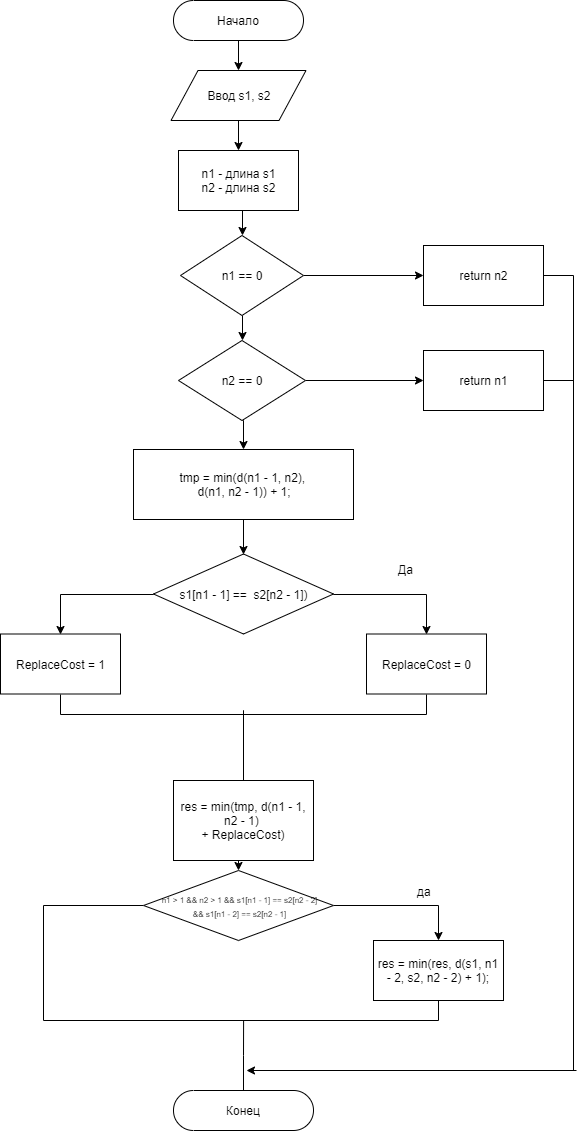
\includegraphics[width=0.75\linewidth]{RecDL.png}
\caption{Схема рекурсивного алгоритма нахождения расстояния Дамерау-Левенштейна}
\label{fig:mpr}
\end{figure}


\chapter{Технологическая часть}
\section{Выбор ЯП}
Для реализации программ я выбрал язык программирования Java, так имею большой опыт работы с ним. Среда разработки - Intellij IDEA.

\section{Реализация алгоритма}

\begin{lstlisting}[label=some-code,caption=Класс нахождения расстояния Левенштейна матрично]
public class LowensteinDistance extends DistanceBase {
    protected int[][] matrix;

    public LowensteinDistance(String firstWord, String secondWord) {
        super(firstWord, secondWord);
    }

    @Override
    protected int calculateDistance() {
        matrix = new int[firstWord.length() + 1][secondWord.length() + 1];
        fillMatrix();
        findDistanceInMatrix();
        return getResultFromMatrix();
    }

    protected void getNextElementInMatrix(int i, int j) {
        int cost = calculateCost(i, j);

        matrix[i][j] = Math.min(Math.min(matrix[i - 1][j] + 1, matrix[i][j - 1] + 1), matrix[i - 1][j - 1] + cost);
    }

    protected int calculateCost(int i, int j) {
        return (firstWord.charAt(i - 1) == (secondWord.charAt(j - 1))) ? 0 : 1;
    }

    private void findDistanceInMatrix() {
        for (int i = 1; i <= firstWord.length(); i++) {
            for (int j = 1; j <= secondWord.length(); j++) {
                getNextElementInMatrix(i, j);
            }
        }
    }

    private void fillMatrix() {
        fillMatrixFirstColumn();
        fillMatrixFirstRow();
    }

    private void fillMatrixFirstColumn() {
        for (int i = 0; i < firstWord.length() + 1; i++) {
            matrix[i][0] = i;
        }
    }

    private void fillMatrixFirstRow() {
        for (int i = 0; i < secondWord.length() + 1; i++) {
            matrix[0][i] = i;
        }
    }

    private int getResultFromMatrix() {
        return matrix[firstWord.length()][secondWord.length()];
    }

    @Override
    public String toString() {

        StringBuilder distanceMatrix = new StringBuilder("\n\n");
        for (int i = 0; i < matrix.length; i++)
        {
            for (int j = 0; j < matrix.length; j++)
                distanceMatrix.append(matrix[i][j] + "\t");
            distanceMatrix.append("\n");
        }
        distanceMatrix.append("\n\n");

        return distanceMatrix.toString();
    }
}
\end{lstlisting}


\begin{lstlisting}[label=some-code,caption=Класс нахождения расстояния Дамерау-Левенштейна матрично]
public class LowensteinDamerauDistance extends LowensteinDistance {
    public LowensteinDamerauDistance(String firstWord, String secondWord) {
        super(firstWord, secondWord);
    }

    @Override
    protected void getNextElementInMatrix(int i, int j) {
        super.getNextElementInMatrix(i, j);

        if (adjacentLetterEqual(i, j))
            matrix[i][j] = Math.min(matrix[i][j], matrix[i - 2][j - 2] + calculateCost(i, j));
    }

    private boolean adjacentLetterEqual(int i, int j) {
        if (i > 1 && j > 1 &&
                firstWord.charAt(i - 1) == secondWord.charAt(j - 2) &&
                firstWord.charAt(i - 2) == secondWord.charAt(j - 1)) {
            return true;
        }
        return false;
    }
}
\end{lstlisting}


\begin{lstlisting}[label=some-code,caption=Класс нахождения расстояния Дамерау-Левенштейна рекурсивно]
public class LowensteinRecursiveDistance extends DistanceBase {
    public LowensteinRecursiveDistance(String firstWord, String secondWord) {
        super(firstWord, secondWord);
    }

    @Override
    protected int calculateDistance() {
        return calculateRecursive(firstWord.length(), secondWord.length());
    }

    private int calculateRecursive(int firstWordLength, int secondWordLength) {
        int cost;

        if (firstWordLength == 0)
            return secondWordLength;
        if (secondWordLength == 0)
            return firstWordLength;

        if (firstWord.charAt(firstWordLength - 1) == secondWord.charAt(secondWordLength - 1))
            cost = 0;
        else
            cost = 1;


        return Collections.min(Arrays.asList(
                calculateRecursive(firstWordLength - 1, secondWordLength) + 1,
                calculateRecursive(firstWordLength, secondWordLength - 1) + 1,
                calculateRecursive(firstWordLength - 1, secondWordLength - 1) + cost
        ));
    }
}
\end{lstlisting}


\chapter{Исследовательская часть}

\section{Сравнительный анализ на основе замеров времени работы алгоритмов}

Был проведен замер времени работы каждого из алгоритмов.


\begin{table} [h!]
\centering
\caption{Время работы алгоритмов (в милисекундах)}
	\begin{tabular}{|c c c c|} 
 	\hline
	len & Lev(M) & DamLev(M)  & DamLev(R) \\ [0.8ex] 
 	\hline\hline
 	3 & 2 & 4 & 309\\
 	\hline
 	4 & 3 & 5 & 434\\
 	\hline
	5 & 3 & 3 & 572\\
	\hline
	6 & 5 & 5 & 867\\
	\hline
	7 & 6 & 7 & 1004\\
	\hline
	\end{tabular}
\end{table}


\begin{tikzpicture}

\begin{axis}[
    	axis lines = left,
    	xlabel={len (symbols)},
    	ylabel={time (ms)},
    	xmin=3, xmax=7,
    	ymin=1, ymax=1500,
	legend pos=north west,
	ymajorgrids=true
]
\addplot[color=orange] table[x index=0, y index=1] {DamLevR.dat};
\addplot[color=blue, mark=square] table[x index=0, y index=1] {LevM.dat};
\addplot[color=green, mark=square] table[x index=0, y index=1] {DamLevM.dat};

\addlegendentry{DamLevR}
\addlegendentry{LevT}
\addlegendentry{DamLevT}
\end{axis}
\end{tikzpicture}


\par
Наиболее эффективными по времени являются матричные реализации алгоритмов, уже при длине строк в 7 символов выигрышность становится более чем в 1,000 раз. Это обусловлено большим количеством повторных рассчетов рекурсивных алгоритмов. Время работы алгоритма, использующего матрицу, намного меньше благодаря тому, что в нем требуется только (m + 1)*(n + 1) операций заполнения ячейки матрицы. Также установлено, что алгоритм ДамерауЛевенштейна работает немного дольше алгоритма Левенштейна, т.к. в нем добавлены дополнительные проверки, однако алгоритмы сравнимы по временной эффективности.


\section{Сравнительный анализ на основе замеров потребляемой памяти алгоритмов}
\par Для проведения анализа замерим потребляемую память у разных реализаций алгоритма. Все измерения представлены в байтах

\begin{table} [h!]
\centering
\caption{Потребляемая память структурами данных в алгоритме нахождения расстояния Левенштейна}
	\begin{tabular}{|c c c|} 
 	\hline
	Структура данных & Длина 4 символа & Длина 1000 символов\\ [0.8ex] 
 	\hline\hline
 	Матрица & 480 & 8064096\\
 	\hline
 	Две вспомогательные переменные (int) & 56 & 56\\
 	\hline
	Два счетчика (int) & 56 & 56\\
	\hline
	Передача параметров & 106 & 2098\\
	\hline
	Cумма данных & 698 & 8066306\\
	\hline
	\end{tabular}
\end{table}

\begin{table} [h!]
\centering
\caption{Потребляемая память структурами данных в алгоритме нахождения расстояния Дамерау-Левенштейна}
	\begin{tabular}{|c c c|} 
 	\hline
	Структура данных & Длина 4 символа & Длина 1000 символов\\ [0.8ex] 
 	\hline\hline
 	Матрица & 480 & 8064096\\
 	\hline
 	Три вспомогательные переменные (int) & 84 & 84\\
 	\hline
	Два счетчика (int) & 56 & 56\\
	\hline
	Передача параметров & 106 & 2098\\
	\hline
	Cумма данных & 726 & 8066334\\
	\hline
	\end{tabular}
\end{table}

\begin{table} [h!]
\centering
\caption{Потребляемая память структурами данных в рекурсивном алгоритме нахождения расстояния Дамерау-Левенштейна}
	\begin{tabular}{|c c c|} 
 	\hline
	Структура данных & Длина 4 символа & Длина 1000 символов\\ [0.8ex] 
 	\hline\hline
 	Пять переменных для подсчета IDTR & 140 * 4 = 560 & 140 * 1000 = 140000\\
 	\hline
	Передача параметров & 106 * 8 = 848 & 2098 * 2000 = 4196000\\
	\hline
	Cумма данных & 1408 & 4336000\\
	\hline
	\end{tabular}
\end{table}



\par
Таким образом, рекурсивный алгоритм занимает примерно одинаковое кол-во памяти при маленькой длине строк, и значительно выигрывает при строках большего размера.


\section{Тестовые данные}

\par
Проведем тестирование программы. В столбцах "Ожидаемый результат" и "Полученный результат" 3 числа соответсвуют матричному алгоритму нахождению расстоянию Левенштейна, рекурсивному алгоритму расстояния Дамерау-Левенштейна, матричному алгоритму нахождения расстояние Дамерау-Левенштейна.

\begin{table} [h!]
\caption{Таблица тестовых данных}
	\begin{tabular}{|c c c c c|} 
 	\hline
	№ & Первое слово & Второе слово & Ожидаемый результат & Полученный результат \\ [0.8ex] 
 	\hline\hline
 	1 &  &  & 0 0 0 & 0 0 0\\
 	\hline
 	2 & kot & skat & 2 2 2 & 2 2 2\\
 	\hline
	3 & kate & ktae & 2 1 1 & 2 1 1\\
	\hline
	4 & abacaba & aabcaab & 4 2 2 & 4 2 2\\
	\hline
	5 & sobaka & sboku & 3 3 3 & 3 3 3\\
	\hline
	6 & qwerty & queue & 4 4 4 & 4 4 4\\
	\hline
	7 & apple & aplpe & 2 1 1  & 2 1 1\\
	\hline
	8 &  & cat & 3 3 3 & 3 3 3\\
	\hline
	9 & parallels &  & 9 9 9 & 9 9 9\\
	\hline
	10 & bmstu & utsmb & 4 4 4 & 4 4 4\\
	\hline
	\end{tabular}
\end{table}



\chapter*{Заключение}
\addcontentsline{toc}{chapter}{Заключение}
Был изучен метод динамического программирования на материале алгоритмов Левенштейна и Дамерау-Левенштейна.
Также изучены алгоритмы Левенштейна и Дамерау-Левенштейна нахождения расстояния между строками, получены практические навыки раелизации указанных алгоритмов
в матричной  и рекурсивных версиях. 

Экспериментально было подтверждено различие во временной эффективности рекурсивной и нерекурсивной реализаций выбранного алгоритма определения расстояния между строками при помощи разработаного программного обеспечения на материале замеров времени выполнения реализации на варьирующихся длинах строк. 

В результате исследований я пришел к выводу, что матричная реализация данных алгоритмов заметно выигрывает по времени при росте длины строк, следовательно более применима в реальных проектах.


\end{document}